\documentclass[12pt, a4paper]{article}

\usepackage{amssymb}
\usepackage{amsthm}
\usepackage{amscd}
\usepackage{amsmath}
\usepackage{enumitem}
\usepackage{multicol, fullpage}
\usepackage{amsfonts,epsfig,epstopdf,titling,url,array}
\usepackage{esint} %Lines up double+ integrals


\usepackage[usenames,dvipsnames]{xcolor} % allows you to use color names, call this BEFORE you call TikZ

\usepackage{tikz, tikz-3dplot, pgfplots}
\usepackage{tkz-graph}
\usetikzlibrary{hobby}
\pgfplotsset{compat=1.8}

% formatting the section titles
\usepackage{titlesec}
\titleformat{\section}{\large\bfseries}{\thesection}{1em}{}

\usetikzlibrary{calc}




\setlength{\evensidemargin}{1in}
\addtolength{\evensidemargin}{-1in}
\setlength{\oddsidemargin}{1.5in}
\addtolength{\oddsidemargin}{-1.5in}
\setlength{\topmargin}{1in}
\addtolength{\topmargin}{-1.5in}

\setlength{\textwidth}{16cm}
\setlength{\textheight}{23cm}


\theoremstyle{plain}

\newtheorem{theorem}{Theorem}[section]
\newtheorem{lemma}{Lemma}
\newtheorem{proposition}{Proposition}
\newtheorem*{corollary}{Corollary}

\theoremstyle{definition}

\newtheorem{definition}{Definition}[section]
\newtheorem{notation}{Notation}
\newtheorem{question}{Question}
\newtheorem{conjecture}{Conjecture}[section]
\newtheorem{solution}{Solution}[section]
\newtheorem{example}{Example}[section]
\newtheorem{counter}{Counter Example}[section]


\theoremstyle{remark}
\newtheorem*{rem}{Remark}
\newtheorem*{note}{Note}



\def\proof{\noindent {\it Proof.} \hskip 0.1in}
\def\qed{\rightline{$\blacklozenge$}}

\newcommand{\RR}{\mathbb{R}}
\newcommand{\QQ}{\mathbb{Q}}
\newcommand{\NN}{\mathbb{N}}
\newcommand{\ZZ}{\mathbb{Z}}
\newcommand{\CC}{\mathbb{C}}
\newcommand{\II}{\mathbb{I}}






\begin{document}
\author{Sean Kearns}

\begin{minipage}{0.4\textwidth}
\begin{flushleft}
Sean Kearns\\
\today
\end{flushleft}
\end{minipage}
\begin{minipage}{0.4\textwidth}
\begin{flushright}
MATH5470\\
Vector Calculus Notes
\end{flushright}
\end{minipage}



\tableofcontents











\newpage
\part{Vector Calculus}




\section{Displacement Vectors}

\begin{definition}
The \textbf{displacement vector} from one point to another is an arrow with its tail at the first point and its tip at the second.  The \textbf{magnitude} (or length) of the displacement vector is the distance between the points, and is represented by the length of the arrow.  The \textbf{direction} of the displacement vector is the direction of the arrow.
\end{definition}

\begin{definition}
Displacement vectors which point in the same direction and have the same magnitude are considered to be the same, even if they do not coincide.
\end{definition}

\begin{definition}
A quantity specified only by a number, but no direction, is called a \textbf{scalar}.
\end{definition}

\begin{definition}
The \textbf{sum}, $\vec{v}$ $+$ $\vec{w}$, of two vectors $\vec{v}$ and $\vec{w}$ is the combined displacement resulting from first applying $\vec{v}$ and then $\vec{w}$.  The sum $\vec{w}$ $+$ $\vec{v}$ gives the same displacement.
\end{definition}

\begin{center}
\begin{tikzpicture}[scale=1.6]
	 
	% draw axes
	
	\draw (-1,0) -- (2,0) node[anchor=north east]{$x$};
	\draw (0,-1) -- (0,2) node[anchor=north west]{$y$};

	% simple roots

	\draw[line width=1,color=blue,->] (2,-1) -- (0,0) node[anchor=north east]{$\vec{w}$};
	\draw[line width=1,color=blue,->] (0,0) -- (0,1) node[anchor=north east]{$\vec{v}$};
	\draw[line width=1,color=red,->] (2,-1) -- (0,1) node[anchor=south]{$\vec{w}+\vec{v}$};


	
	
	\node[rectangle,draw] at (-3,0) {Vector Sum};
	
\end{tikzpicture}
\end{center}

\begin{definition}
The \textbf{difference}, $\vec{w}$ $-$ $\vec{v}$, is the displacement vector which, when added to $\vec{v}$, gives $\vec{w}$.  That is, $\vec{w}$ $=$ $\vec{v}$ $+$ ($\vec{w}$ $-$ $\vec{v}$).
\end{definition}

\begin{center}
\begin{tikzpicture}[scale=1.6]
	 
	% draw axes
	
	\draw (-1,0) -- (2,0) node[anchor=north east]{$x$};
	\draw (0,-1) -- (0,2) node[anchor=north west]{$y$};

	% simple roots

	\draw[line width=1,color=blue,->] (0,0) -- (2,-1) node[anchor=north east]{$\vec{w}$};
	\draw[line width=1,color=blue,->] (0,0) -- (0,1) node[anchor=north east]{$\vec{v}$};
	\draw[line width=1,color=red,->] (0,1) -- (2,-1) node[anchor=west]{$\vec{w}-\vec{v}$};


	
	
	\node[rectangle,draw] at (-3,0) {Vector Difference};
	
\end{tikzpicture}
\end{center}

\begin{definition}
The \textbf{zero vector}, $\vec{0}$, is a displacement vector with zero length.
\end{definition}

\begin{definition}
If $\lambda$ is a scalar and $\vec{v}$ is a displacement vector, the \textbf{scalar multiple of} $\vec{v}$ \textbf{by} $\lambda$, written $\lambda$$\cdot$$\vec{v}$, is the displacement vector with the following properties $1$ and $2$.
\end{definition}

\begin{definition}
The displacement vector $\lambda$$\cdot$$\vec{v}$ is parallel to $\vec{v}$, pointing in the same direction if $\lambda$$>$$0$, and in the opposite direction if $\lambda$$<$$0$ (1).
\end{definition}

\begin{definition}
The magnitude of $\lambda$$\cdot$$\vec{v}$ is $|\lambda|$ times the magnitude of $\vec{v}$, that is, $||\lambda \cdot \vec{v}||$ $=$ $|\lambda| \cdot ||\vec{v}||$ (2).
\end{definition}

\begin{definition}
Two vectors $\vec{v}$ and $\vec{w}$ are \textbf{parallel} if one is a scalar multiple of the other, that is, if $\vec{w}$ $=$ $\lambda$$\cdot$$\vec{v}$.
\end{definition}



\begin{definition}
Vectors are closed under vector addition and scalar multiplication.  
\end{definition}


\begin{definition}
We \textbf{resolve} $\vec{v}$ into components by writing $\vec{v}$ in the form
$$ \vec{v} = v_1 \hat{i} + v_2 \hat{j} + v_3 \hat{k}. $$
We call $v_1 \hat{i}$, $v_2 \hat{j}$, and $v_3 \hat{k}$ the \textbf{components} of $\vec{v}$.
\end{definition}

\begin{center}
\tdplotsetmaincoords{80}{110}
\begin{tikzpicture}[tdplot_main_coords, scale=1.8]
	 
	\coordinate (O) at (0,0,0);
	\tdplotsetcoord{P}{1}{-100}{200}
	
	\draw[thick,->] (0,0,0) -- (5,0,0) node[anchor=north east]{$x$};
	\draw[thick,->] (0,0,0) -- (0,2.5,0) node[anchor=north west]{$y$};
	\draw[thick,->] (0,0,0) -- (0,0,2) node[anchor=south]{$z$};

	\draw[line width=1,color=red,->] (3,0,0) -- (3,2,2) node[anchor=west]{$ \vec{v} = <3,2,2> \;$};
	\draw[line width=1,color=blue,->] (0,0,0) -- (3,0,0) node[anchor=east]{$ 3 \hat{i} \;$};
	\draw[line width=1,color=blue,->] (0,0,0) -- (0,2,0) node[anchor=south west]{$ 2 \hat{j} \;$};
	\draw[line width=1,color=blue,->] (0,0,0) -- (0,0,2) node[anchor=east]{$ 2 \hat{k} \;$};
\end{tikzpicture}
\end{center}
where $v_1=3$, $v_2=2$, and $v_3=2$.
\begin{definition}
The displacement vector from the point $P_1 = (x_1, y_1, z_1)$ to the point $P_2 = (x_2, y_2, z_2)$ is given in components by 
$$ \vec{P}_{1,2} = (x_2-x_1)\hat{i} + (y_2-y_1)\hat{j} + (z_2-z_1)\hat{k} $$
\end{definition} 




\begin{center}
\tdplotsetmaincoords{80}{110}
\begin{tikzpicture}[tdplot_main_coords, scale=1.8]
	 
	\coordinate (O) at (0,0,0);
	\tdplotsetcoord{P}{1}{-100}{200}
	
	\draw[thick,->] (0,0,0) -- (5,0,0) node[anchor=north east]{$x$};
	\draw[thick,->] (0,0,0) -- (0,2.5,0) node[anchor=north west]{$y$};
	\draw[thick,->] (0,0,0) -- (0,0,2) node[anchor=south]{$z$};

	\draw[line width=1,color=red,->] (3,0,0) -- (3,2,2) node[anchor=east]{$ \vec{P}_{1,2} \;$};
	\draw[line width=1,color=blue,->] (0,0,0) -- (1,0,0) node[anchor=east]{$ \hat{i} \;$};
	\draw[line width=1,color=blue,->] (0,0,0) -- (0,1,0) node[anchor=south west]{$ \hat{j} \;$};
	\draw[line width=1,color=blue,->] (0,0,0) -- (0,0,1) node[anchor=east]{$ \hat{k} \;$};
	%\draw[fill=black] (2,0,0) circle (.05);
	\node at (3,0,0) {$P_1 \quad \quad \quad $};
	\node at (3,0,0) {$\bullet$};
	\node at (3,2,2) {$\bullet$};
	\node at (3,2,2) {$\quad \quad \quad P_2$};
\end{tikzpicture}
\end{center}
















\newpage
\subsection{Velocity Vectors and General Properties}

\begin{definition}
The \textbf{velocity vector} of a moving object is a vector whose magnitude is the speed of the object and whose direction is the direction of its motion.  
\end{definition}

\begin{definition}
Vector addition is commutative, and associative. That is, for vectors $\vec{u}$, $\vec{v}$, and $\vec{w}$, 
\begin{eqnarray*}
\vec{v}+ \vec{w} &=& \vec{w}+\vec{v} \\
(\vec{u} + \vec{v}) + \vec{w} &=& \vec{u}+ (\vec{v} + \vec{w}) \\
\end{eqnarray*}
\end{definition}

\begin{definition}
Scalar multiplication holds for the distributive laws. That is, for vectors $\vec{u}$, $\vec{v}$, and constants $\alpha , \beta, \in \RR$
\begin{eqnarray*}
(\alpha+\beta) \vec{v} &=& \alpha \vec{v}+ \beta \vec{v} \\
\alpha (\vec{u} + \vec{v}) &=& \alpha \vec{u}+ \alpha \vec{v} \\
\end{eqnarray*}
\end{definition}

\textbf{Vector Identities}
\vspace{.05in}

1. $1\vec{v} = \vec{v} $

2. $0\vec{v} = \vec{0}$
 
3. $\vec{v} + \vec{0} = \vec{v}$
 
4. $\vec{w} + (-1)\vec{v} = \vec{w} - \vec{v} $



\begin{definition}
A vector in n-dimensions can be written as \,
$ \vec{c} = (c_1, c_2, \ldots , c_n)$.
\end{definition}




\section{Dot Product}
\begin{definition}
\begin{itemize}
Where the angle $\theta$ between $\vec{v}$ and $\vec{w}$ such that $0$ $\le$ $\theta$ $\le$ $\pi$, 

\item \textbf{Geometric Definition} 
$$\vec{v} \cdot \vec{w}= ||\vec{v}|| \cdot ||\vec{w}|| \cdot cos(\theta)$$
 and 

\item \textbf{Algebraic Definition} 
$$\vec{v} \cdot \vec{w} = v_1w_1 + v_2w_2 + v_3w_3$$ 
are equivalent. Notice that the dot product of two vectors is a \textbf{number}.
\end{itemize}
\end{definition}




\begin{definition}
The properties of the Dot Product for any vectors $\vec{u}$, $\vec{v}$, and $\vec{w}$ and any scalar $\lambda$ are:
\begin{align*}
\vec{v} \cdot \vec{w} &= \vec{w} \cdot \vec{v} \\
\vec{v} \cdot (\lambda \vec{w}) &=\lambda ( \vec{w} \cdot \vec{v}) = (\lambda \vec{v}) \cdot \vec{w} \\
(\vec{v} + \vec{w}) \cdot \vec{u} &= \vec{v} \cdot \vec{u} +  \vec{w} \cdot \vec{u} \\
\end{align*}
\end{definition}

\begin{definition}
Two nonzero vectors $\vec{v}$ and $\vec{w}$ are \textbf{perpendicular}, or \textbf{orthogonal}, if and only if $$\vec{v} \cdot \vec{w} = 0$$
\end{definition}

\begin{definition}
Magnitude and dot product are related as follows:
$$ \vec{v} \cdot \vec{v} = ||\vec{v}||^2 = \sqrt{v_1^2+v_2^2+v_3^2}.$$
\end{definition}

\begin{definition}
The \textbf{equation of a plane} with normal vector $\vec{n} = a \hat{i} + b \hat{j} + c \hat{k}$ and containing the point $P_0 = (x_0, y_0, z_0)$ is 
$$ a(x-x_0) + b(y-y_0) + c(z-z_0) = 0.$$
Letting $d= ax_0+by_0+cz_0$ (a constant), we can write the equation of the plane in the form 
$$ ax + by + cz = d.$$
\end{definition}


\begin{definition}
The algebraic definition of the dot product can be extended to vectors in higher dimensions. If $\vec{u} = (u_1, \ldots , u_n)$ and $\vec{v} = (v_1, \ldots , v_n)$ ten the dot product of $\vec{u}$ and $\vec{v}$ is the \textbf{scalar}
$$ \vec{u} \cdot \vec{v} = u_1v_1 + \ldots + u_nv_n.$$
\end{definition}

\begin{definition}
The projection of a vector $\vec{v}$ on the line in the direction of the unit vector $\vec{u}$, or 
\begin{align*}
&\vec{v}_{\text{parallel}} = (\vec{v} \cdot \vec{u})\vec{u} \quad \text{where} \quad ||\vec{u}|| = 1 \\
&\vec{v} = \vec{v}_{\text{parallel}} + \vec{v}_{\text{perp}}. \\
\end{align*}
\end{definition}



\begin{center}
\begin{tikzpicture}[scale=1.6]
	 
	% draw axes
	
	\draw (-1,0) -- (2,0) node[anchor=north east]{$x$};
	\draw (0,-1) -- (0,2) node[anchor=north west]{$y$};

	% simple roots

	\draw[line width=1,color=blue,->] (2.35,.8) -- (2,2) node[anchor=west]{$\vec{v}_{\text{perp}}$};
	\draw[line width=1,color=blue,->] (0,0) -- (3,1) node[anchor=west]{$\vec{v}_{\text{parallel}}$};
	\draw[line width=1,color=red,->] (0,0) -- (2,2) node[anchor=east]{$\vec{v}$ \quad};


	
	
	\node[rectangle,draw] at (-3,0) {Vector Projection};
\end{tikzpicture}
\end{center}



\begin{definition}
The \textbf{work}, $W$, done by a force $\vec{F}$ acting on an object through a displacement $\vec{d}$ is given by 
$$ W = (||\vec{F}|| \cos \theta) ||\vec{d}|| = ||\vec{F}|| \, ||\vec{d}|| \cos \theta = \vec{F} \cdot \vec{d}.$$

Note that $\theta = 0$ since the work done in some direction $\vec{v}_{\text{parallel}}$ by some vector $\vec{v}$ is the projection $\it{of}$ $\vec{v}$ onto $\vec{v}_{\text{parallel}}$.

\end{definition}


\newpage

\subsection{Cross Product}

\begin{definition}
The \textbf{right-hand rule} expresses a universal way to orient two vectors with respect to eachother in a plane. Place $\vec{v}$ and $\vec{w}$ so that their tails coincide and curl the fingers of your right hand through the smaller of the two angles from $\vec{v}$ to $\vec{w}$; your thumb points in the direction of the normal vector, $\vec{n}$.
\end{definition}



\begin{center} 
\begin{tikzpicture}[scale=1.6]
	
         \draw (0,0) -- (2,0) node[anchor=north east]{$x$};
	\draw (0,0) -- (0,2) node[anchor=north west]{$y$};

	\draw[fill=Cyan] (0,0) -- (1,0) -- (1.70710678119,1) -- (0.70710678119,1) -- cycle;
	\node at (.1,.1){ \; \; $\theta$};

         \draw[line width=1,color=blue,->] (0,0) -- (1,0) node[anchor=north west]{$\vec{v}$};
	\draw[line width=1,color=blue,->] (0,0) -- (0.70710678119,1) node[anchor=south]{$\vec{w}$};

	\node[rectangle,draw] at (-3,0) {From $\vec{v}$ to $\vec{w}$ in direction $\theta$};

\end{tikzpicture}
\end{center}  

\begin{definition}
The following two definitions of the \textbf{cross product} or \textbf{vector product} $\vec{v} \times \vec{w}$ are equivalent:
\begin{itemize}
\item \textbf{Geometric Definition}
$$  \vec{v} \times \vec{w} = \left( \text{Area of parallelogram with edges} \; \vec{v} \; \text{and} \; \vec{w}  \right) \vec{n} = (||\vec{v}|| \, ||\vec{w}|| sin \theta)\vec{n}, $$
where $0 \le \theta \le \pi$ is the angle between $\vec{v}$ and $\vec{w}$, and $\vec{n}$ is the unit vector perpendicular to $\vec{v}$ and $\vec{w}$ pointing in the direction given by the right-hand rule. If $\vec{v}$ and $\vec{w}$ are parallel, then $\vec{v} \times \vec{w} = \vec{0}$.



\item \textbf{Algebraic Definition}
$$\vec{v} \times \vec{w} = (v_2w_3 - v_3w_2)\hat{i} + (v_3w_1 - v_1w_3)\hat{j} + (v_1w_2 - v_2w_1)\hat{k} $$
where $\vec{v} = v_1 \hat{i} + v_2 \hat{j} + v_3 \hat{k}$ and $\vec{w} = w_1 \hat{i} + w_2 \hat{j} + w_3 \hat{k}$
\end{itemize}
\end{definition}


\[\vec{v} \times \vec{w} = \left( \begin{array}{ccc}
\hat{i} & \hat{j} & \hat{k} \\
v_1     & v_2     & v_3 \\
w_1    & w_2    & w_3
\end{array} \right) = (v_2w_3 - v_3w_2)\hat{i} + (v_3w_1 - v_1w_3)\hat{j} + (v_1w_2 - v_2w_1)\hat{k} \]

\textbf{Properties of the Cross Product}
\vspace{.05in}

For vectors $\vec{u}$, $\vec{v}$, $\vec{w}$, and scalar $\lambda$

1. $\vec{v} \times \vec{w} = -(\vec{w} \times \vec{v})$

2. $(\lambda \vec{v}) \times \vec{w}) = \lambda ( \vec{v} \times \vec{w} ) = \vec{v} \times (\lambda \vec{w})$

3. $\vec{u}(\vec{v} + \vec{w}) = \vec{u} \vec{v} + \vec{u} \vec{w}$

\newpage

\textbf{Area of a parallelogram} with edges $\vec{v} = v_1 \hat{i} + v_2 \hat{j} + v_3 \hat{k}$ and $\vec{w} = w_1 \hat{i} + w_2 \hat{j} + w_3 \hat{k}$ is 

\[ \text{Area} \, = ||\vec{v} \times \vec{w}||, \quad \quad \quad \quad \text{where} \quad \vec{v} \times \vec{w} = \left( \begin{array}{ccc}
\hat{i} & \hat{j} & \hat{k} \\
v_1     & v_2     & v_3 \\
w_1    & w_2    & w_3
\end{array} \right) \]

\begin{center}
\tdplotsetmaincoords{80}{110}
\begin{tikzpicture}[tdplot_main_coords, scale=1.8]
	 
	\coordinate (O) at (0,0,0);
	\tdplotsetcoord{P}{1}{-100}{200}
	
	\draw[thick,->] (0,0,0) -- (5,0,0) node[anchor=north east]{$x$};
	\draw[thick,->] (0,0,0) -- (0,2.5,0) node[anchor=north west]{$y$};
	\draw[thick,->] (0,0,0) -- (0,0,2) node[anchor=south]{$z$};


	\draw[line width=2,color=blue,->] (0,0,0) -- (3,0,0) node[anchor=east]{$\vec{v}$ \quad};
	%\draw[line width=1,color=blue,] (3,0,0) -- (3,2,-1) node[anchor=east]{};
	%\draw[line width=1,color=blue,] (3,2,-1) -- (0,2,-1) node[anchor=east]{};
         \draw[line width=2,color=blue,->] (0,0,0) -- (0,2,-1) node[anchor=south west]{ $\vec{w}$};

     
         \draw[fill=Cyan] (0,0,0) -- (3,0,0) -- (3,2,-1) -- (0,2,-1) -- cycle;
	\node at (.6,.2,-.1){ $\theta$};
\end{tikzpicture}
\end{center}

\vspace{.05in}

\textbf{Volume of a parallelpiped} with edges $\vec{a}$, $\vec{b}$, $\vec{c}$ is given by 

\[ \text{Volume} \, = \left|(\vec{b} \times \vec{c}) \cdot \vec{a} \right|= \quad \text{Absolute value of the determinant} \quad \left( \begin{array}{ccc}
a_1 & a_2 & a_3 \\
b_1 & b_2 & b_3 \\
c_1 & c_2 & c_3
\end{array} \right) \]


\begin{center}
\tdplotsetmaincoords{80}{110}
\begin{tikzpicture}[tdplot_main_coords, scale=1.8]
	 
	\coordinate (O) at (0,0,0);
	\tdplotsetcoord{P}{1}{-100}{200}
	
	\draw[thick,->] (0,0,0) -- (5,0,0) node[anchor=north east]{$x$};
	\draw[thick,->] (0,0,0) -- (0,2.5,0) node[anchor=north west]{$y$};
	\draw[thick,->] (0,0,0) -- (0,0,2) node[anchor=south]{$z$};


	\draw[line width=2,color=blue,->] (0,0,0) -- (3,0,0) node[anchor=east]{$\vec{b}$ \quad};
	\draw[line width=1,color=blue,] (3,0,0) -- (3,2,0) node[anchor=east]{};
	\draw[line width=1,color=blue,] (3,2,0) -- (0,2,0) node[anchor=east]{};
         \draw[line width=2,color=blue,->] (0,0,0) -- (0,2,0) node[anchor=south west]{\quad $\vec{c}$};

         \draw[line width=1,color=blue,] (0,1,1) -- (3,1,1) node[anchor=east]{};
	\draw[line width=1,color=blue,] (3,1,1) -- (3,3,1) node[anchor=east]{};
	\draw[line width=1,color=blue,] (3,3,1) -- (0,3,1) node[anchor=east]{};
         \draw[line width=1,color=blue,] (0,1,1) -- (0,3,1) node[anchor=south west]{};

         \draw[line width=2,color=blue,->] (0,0,0) -- (0,1,1) node[anchor=east]{$\vec{a}$ \quad \quad};
	\draw[line width=1,color=blue,] (3,0,0) -- (3,1,1) node[anchor=east]{};
	\draw[line width=1,color=blue,] (3,2,0) -- (3,3,1) node[anchor=east]{};
         \draw[line width=1,color=blue,] (0,2,0) -- (0,3,1) node[anchor=south west]{};
\end{tikzpicture}
\end{center}
















\newpage
\part{Change of Variables and Integration}

\subsection{Polar Coordinates}

When computing integrals in polar coordinates, use $x=r\cos \theta$, $y=r\sin\theta$, and $x^2+y^2=r^2$. Also, that $dA = r dr d\theta$. Note that this is a 2D transformation.

$$ \int_R f(x, y) \, dA = \int_{\alpha}^{\beta} \int_a^b f(r, \theta) r \, dr \, d\theta$$



\subsection{Cylindrical Coordinates}

Each point in 3-space is represented using $0 \le r < \infty$, $0 \le \theta \le 2\pi$, and $-\infty < z < \infty$ where 
\begin{align*}
&x = r \cos \theta \\
&y = r \sin \theta \\
&z = z.
\end{align*}
As with polar coordinates in the plane, note that $x^2+y^2 = r^2$.

When computing integrals in cylindrical coordinates, $dV = r \, dr \, d\theta \, dz$. Other orders of integration are also possible.

\begin{center}
\tdplotsetmaincoords{80}{100}
\begin{tikzpicture}[tdplot_main_coords, scale=1.8]
	 
	\coordinate (O) at (0,0,0);
	\tdplotsetcoord{P}{1}{-100}{200}
	
	\draw[thick,->] (0,0,0) -- (5,0,0) node[anchor=north east]{$x$};
	\draw[thick,->] (0,0,0) -- (0,2.5,0) node[anchor=north west]{$y$};
	\draw[thick,->] (0,0,0) -- (0,0,2) node[anchor=south]{$z$};

         \draw[color=Cyan,dashed] (0,0,0) -- (4,2,0) ;
         \draw[color=Cyan,dashed] (4,2,0) -- (4,2,2) ;
         \node at (4,2,2){$\bullet$};
         \node at (4,2,2.25){$P = (r, \theta, z)$};
         \node at (4,2,0){$\bullet$};
         \node at (4,2,-.25){$(r, \theta, 0)$};

         \node at (3,2,1){$z$};
         \node at (3,1,0){$r$};
         \draw[->] (1,0) .. controls (1.55,.25) and (1.55,.35) .. (1,.5);
         \node at (.7,.15,0){$\theta$};

\end{tikzpicture}
\end{center}




\subsection{Spherical Coordinates}

Each point in 3-space is represented using $0 \le \rho < \infty$, $0 \le \phi \le \pi$, and $0 \le \theta \le 2\pi$ where 
\begin{align*}
&x = \rho \sin \phi \cos \theta \\
&y = \rho \sin \phi \sin \theta \\
&z = \rho \cos \phi.
\end{align*}
Also, note that $x^2+y^2 + z^2 = \rho^2$.

When computing integrals in spherical coordinates, $dV = \rho^2 \sin \phi \, d\rho \, d\phi \, d\theta dz$. Other orders of integration are also possible. It is important to note that $\phi$ starts from the positive $z$-axis, and moves downward.

\begin{center}
\tdplotsetmaincoords{80}{100}
\begin{tikzpicture}[tdplot_main_coords, scale=1.8]
	 
	\coordinate (O) at (0,0,0);
	\tdplotsetcoord{P}{1}{-100}{200}
	
	\draw[thick,->] (0,0,0) -- (5,0,0) node[anchor=north east]{$x$};
	\draw[thick,->] (0,0,0) -- (0,2.5,0) node[anchor=north west]{$y$};
	\draw[thick,->] (0,0,0) -- (0,0,2) node[anchor=south]{$z$};

         \draw[color=Cyan,dashed] (0,0,0) -- (4,2,0) ;
         \draw[color=Cyan,dashed] (4,2,0) -- (4,2,2) ;
         \draw[color=Cyan] (0,0,0) -- (4,2,2) ;

         \node at (4,2,2){$\bullet$};
         \node at (4,2,2.25){$P = (\rho, \phi, \theta)$};



         \node at (3,1.35,1.1){$\rho$};
         \node at (2.45,.55,0){$\theta$};



         \draw[->] (1,0) .. controls (1.55,.25) and (1.55,.35) .. (1,.5);

         \draw[->] (0,0,.5) .. controls (0,.185,.65) and (0,.365,.65) .. (0,.5,.5);
         \node at (.7,.35,.5){$\phi$};

\end{tikzpicture}
\end{center}





\subsection{Coordinate Transformations in General}

To convert an integral from $x,y$ to $s,t$ coordinates we make three changes:

\begin{enumerate}
\item Substitute for $x$ and $y$ in the integrand in terms of $s$ and $t$ (i.e. $f(x,y) = f(x(s,t),y(s,t))$).
\item Change the $xy$ region $R$ into an $st$ region $T$.
\item Use the absolute value of the Jacobian to change the area element by making the substitution

$ dxdy = \left| \frac{\partial (x,y)}{\partial (s,t)}  \right| \, dsdt$
so that we receive $$\int_R f(x,y) dA = \int_T f(x(s,t),y(s,t)) \left| \frac{\partial (x,y)}{\partial (s,t)}  \right| \, dsdt.$$
\end{enumerate}












\newpage
\part{Parameterization and Vector Fields }










\subsection{Parameterized Curves}

In the following sections it will be valuable to know that $\vec{v} \equiv$ \textbf{v}. 

If we start with a line $L$ that contains a point $P_0 = (x_0, y_0, z_0)$, and is parallel to the vector \textbf{v}, then we may create a component-wise representation of $L$ where $L$ is traced out by the tip of the vector as time varies.

That is,  $\langle x, y, z \rangle = \langle x_0+at, y_0+bt, z_0+ct \rangle $ for $t\in\RR$. Since two vectors are only equal iff their corresponding components are equal, we have
$$ x=x_0+at \quad \quad y=y_0+bt \quad \quad z=z_0+ct $$
These equations are called \textbf{parametric equations} of the line $L$ through the point  $P_0 = (x_0, y_0, z_0)$ and parallel to the vector \textbf{v} $= \langle a, b, c \rangle$. Each value of the parameter $t$ gives a point $(x, y, z)$ on $L$.

The notation \textbf{r} $=$ \textbf{r}$_0 +t$\textbf{v} is a parametric equation of a line $L$ in vector form, and is used as the general parameterization where \textbf{r} $ = \langle x, y, z \rangle$, \textbf{r}$_0 = \langle x_0, y_0, z_0 \rangle$, and \textbf{v} $= \langle a, b, c \rangle$.

\begin{definition}
The line segment from \textbf{r}$_0$ to \textbf{r}$_1$ is given by the vector equation 
$$ \textbf{r}(t) = (1-t)\textbf{r}_0+t\textbf{r}_1 \quad \quad \quad 0 \le t \le 1.$$
\end{definition}

\begin{definition}
A \textbf{normal vector} $\vec{n}$ is a vector orthogonal to a given surface. In particular, one that may be represented as a plane over each infinitesimal area (i.e. smooth continuous surface).
\end{definition}

\begin{definition}
A \textbf{scalar equation} of the plane through $P_0 = (x_0, y_0, z_0)$ with normal vector \textbf{n}$ = \langle a, b, c \rangle$ is as follows:
$$ a(x-x_0) + b(y-y_0) + c(z-z_0) = 0.$$
\end{definition}

\vspace{.05in}

\textbf{Constructing a Unit Normal Vector from a Smooth Surface}

Given a surface $z=g(x,y)$, let us define the function $f(x,y,z) = z-g(x,y)$. Recall that $\nabla f$ will be orthogonal (or normal) to the surface given by $f(x,y,z)=0$. To be sure that we have a unit normal vector we can simply divide by the magnitude of $\nabla f$. That is, 

$$ \hat{n} = \frac{\nabla f}{|| \nabla f ||} = \frac{-g_x \hat{i} -g_y \hat{j} + \hat{k}}{\sqrt{(g_x)^2+(g_y)^2+1}}$$

Note that because the $z$ component is positive, this normal will be in the positive $z$ (or $k$) direction in general.

If our surface is given parametrically as $\vec{r}(s,t) = x(s,t) \hat{i} + y(s,t) \hat{j} + z(s,t) \hat{k}$, where $\vec{r}_s \times \vec{r}_t$ is a tangential plane at a particular point on our surface, and since a vector normal to the tangent plane will be tangent to the surface at any given point, one of the unit normal vectors for the surface will be 

$$\hat{n} = \frac{\vec{r}_s \times \vec{r}_t}{|| \vec{r}_s \times \vec{r}_t ||} $$

As with the first case we will need to look at this once it’s computed and determine if it points in the correct direction or not.  If it doesn’t then we can always take the negative of this vector and that will point in the correct direction.

\vspace{.05in}

\begin{definition}
Two planes are \textbf{parallel} if their normal vectors are parallel.
\end{definition}












\subsection{Motion, Velocity, and Acceleration}

\begin{definition}
The \textbf{velocity vector} of a moving objct is a vector $\vec{v}$ such that:

$\bullet$ The magnitude of $\vec{v}$ is the speed of the object.

$\bullet$ The direction of $\vec{v}$ is the direction of motion.

Thus the speed of the object is $||\vec{v}||$ and the velocity vector is tangent to the object's path.
\end{definition}

\begin{definition}
The \textbf{velocity vector}, $\vec{v}(t)$, of a moving object with position vector $\vec{r}(t)$ at time $t$ is 
$$ \lim_{\Delta t \to 0} \frac{\Delta \vec{r}}{\Delta \vec{t}} = \lim_{\Delta t \to 0} \frac{\vec{r}( t + \Delta \vec{t})-\vec{r}(t)}{\Delta \vec{t}} $$
whenever the limit exists. We use the notation $\vec{v} = \frac{d\vec{r}}{dt} = \vec{r} \, '(t)$.
\end{definition}

\begin{definition}
The \textbf{components of the velocity vector} of a particle moving in space with position vector $\vec{r}(t) = f(t) \hat{i} + g(t) \hat{j} + h(t) \hat{k}$ at time $t$ are given by 

$$\vec{v}(t) = f'(t) \hat{i} + g'(t) \hat{j} + h'(t) \hat{k} = \frac{dx}{dt} \hat{i} + \frac{dy}{dt} \hat{j} + \frac{dz}{dt} \hat{k}. $$
\end{definition}

\begin{definition}
The \textbf{acceleration vector} of an object moving with velocity $\vec{v}(t)$ at time $t$ is
$$ \vec{a}(t) = \lim_{\Delta t \to 0} \frac{\Delta \vec{v}}{\Delta \vec{t}} = \lim_{\Delta t \to 0} \frac{\vec{v}( t + \Delta \vec{t})-\vec{v}(t)}{\Delta \vec{t}} $$
whenever the limit exists. We use the notation $\vec{a} = \frac{d\vec{v}}{dt}  = \frac{d^2 \vec{r}}{dt^2}= \vec{r} \, ''(t)$.
\end{definition}

\begin{definition}
The \textbf{components of the acceleration vector}, $\vec{a}(t)$, at time $t$ of a particle moving in space with position vector $\vec{r}(t) = f(t) \hat{i} + g(t) \hat{j} + h(t) \hat{k}$ at time $t$ are given by 

$$\vec{a}(t) = f''(t) \hat{i} + g''(t) \hat{j} + h''(t) \hat{k} = \frac{d^2x}{dt^2} \hat{i} + \frac{d^2y}{dt^2} \hat{j} + \frac{d^2z}{dt^2} \hat{k}. $$
\end{definition}

\textbf{Uniform Circular Motion}: For a particle whose motion is described by 
$$ \vec{r}(t) = R \cos (\omega t) \hat{i} + R \sin (\omega t) \hat{j}$$

$\bullet$ Motion is in a circle of radius $R$ with period $\frac{2 \pi}{ |\omega|}$.

$\bullet$ Velocity, $\vec{v}$, is tangent to the circle and speed is constant $||\vec{v}|| = |\omega| R$.

$\bullet$ Acceleration, $\vec{a}(t)$, points toward the center of the circle with $||\vec{a}|| = \frac{||\vec{v}||^2}{R}$.


\textbf{Motion in a Straight Line}: For a particle whose motion is described by 
$$ \vec{r}(t) = \vec{r}_0 + f(t) \vec{v}_0$$

$\bullet$ Motion is along a straight line through the point with position vector $\vec{r}_0$ parallel to $\vec{v}_0$.

$\bullet$ Velocity, $\vec{v}$, and acceleration, $\vec{a}$, are parallel to the line.


\begin{definition}
If the curve $C$ is given parametrically for $a \le t \le b$ by smooth functions, and if the velocity vector $\vec{v}$ is not $\vec{0}$ for $a < t < b$, then 
$$ \text{Length of} \; C = \int_a^b ||\vec{v}|| \,dt$$
\end{definition}













\newpage

\subsection{Vector Fields}

\begin{definition} Let $D$ be a set in $\RR^2$ (a plane region). A $\textbf{vector field on} \; \RR^2$ is a function $\textbf{F}$ that assigns to each point $(x,y)$ in $D$ a two-dimensional vector $\textbf{F}(x,y)$.
\end{definition}

\begin{tikzpicture}
    \begin{axis}[
        title={$\textbf{F}(x,y) = \frac{xy}{2}$},
        domain=-2:2,
        view={0}{90},
        axis background/.style={fill=white},
    ]
        \addplot3[blue,
            quiver={
             u={.5*x*y},
             v={.5*x*y},
             scale arrows=0.3,
            },
            -stealth,samples=15]
                {2*x*y};
    \end{axis}
\end{tikzpicture}

\begin{definition} Let $E \subseteq \RR^3$. A \textbf{vector field on} $ \RR^3$ is a function \textbf{F} that assigns to each point $(x, y, z)$ in $E$ a three-dimensional vector $\textbf{F}(x, y, z)$.
\end{definition}


\begin{definition} The gradient $\nabla  f$ (or grad $f$) is defined by 
$$ \nabla f(x, y) = f_x(x, y) \hat{i} + f_y(x, y) \hat{j}$$
in $\RR^2$, and as follows in $\RR^3$:

$$ \nabla f(x, y, z) = f_x(x, y, z) \hat{i} + f_y(x, y, z) \hat{j} +f_z(x, y, z) \hat{k}$$

It is important to note that $\nabla f$ can be called a \textbf{gradient vector field}.
\end{definition}

\begin{tikzpicture}
    \begin{axis}[
        title={$\nabla f = \frac{y}{2} \hat{i} + \frac{x}{2} \hat{j}$ },
        domain=-2:2,
        view={0}{90},
        axis background/.style={fill=white},
    ]
        \addplot3[blue,
            quiver={
             u={.5*y},
             v={.5*x},
             scale arrows=0.3,
            },
            -stealth,samples=15]
                {2*x*y};
    \end{axis}
\end{tikzpicture}

\begin{definition} A vector field \textbf{F} is called a \textbf{conservative vector field} if it is the gradient of some scalar function. In other words, if there exists a function $f$ such that $\textbf{F} = \nabla f$. $f$ is called a \textbf{potential function} for \textbf{F}.
\end{definition}

\begin{definition}
A \textbf{flow line} of a vector field $\vec{v} = \textbf{F}(\vec{r})$ is a path $\vec{r}(t)$ whose velocity vector equals $\vec{v}$. Thus 
$$\vec{r} \, '(t) = \vec{v} = \textbf{F}(\vec{r}(t)). $$
The \textbf{flow} of a vector field is the family of all of the vector field's flow lines.
\end{definition}


\textbf{Parametric Equations for a Plane}

The plane through the point with position vector $\vec{r}_0$ and containing the two $\it{nonparallel}$ vectors $\vec{v}_1$ and $\vec{v}_2$ has parametric equation
$$ \vec{r}(s, t) = \vec{r}_0 + s\vec{v}_1 + t\vec{v}_2.$$




















\newpage
\part{Line Integrals}


\begin{definition}
A curve is said to be \textbf{oriented} if we have chosen a direction of travel on it.
\end{definition}

\begin{definition} If $f$ is defined on a smooth curve $C$ given by the parameterizations $x=x(t)$, and $y=y(t)$ for $a \le t \le b$, then the \textbf{line integral of $f$ along $C$} is 

$$ \int_C f(x, y) \,ds = \lim_{n\to\infty} \sum_{i=0}^{n-1} f(x_i^*, y_i^*) \Delta s_i $$
if the limit exists. 
\end{definition}

We know that the arclength $L$ of a curve $C$ is defined by 

$$ L =  \int_a^b \sqrt{ \left( \frac{dx}{dt}^2  \right) + \left( \frac{dy}{dt}^2  \right)} \, dx  $$

and assuming that $f$ is continuous we may parameterize the previous definition as follows:

$$ \int_C f(x, y) \,ds = \int_a^b f(x(t), y(t)) \sqrt{ \left( \frac{dx}{dt}^2  \right) + \left( \frac{dy}{dt}^2  \right)} \, dx$$

which an be written in vector notation like so:

$$ \int_a^b f(\vec{r}(t)) |\vec{r} \, '(t)| \, dt $$


\begin{definition} Let \textbf{F} be a continuous vector field defined on a smooth curve $C$ given by a vector function $\vec{r}(t)$, for $a \le t \le b$. Then the \textbf{line integral of F along C} is 

$$ \int_C \textbf{F} \cdot d \textbf{r} = \lim_{||\Delta \vec{r}_i ||\to 0} \sum_{i=0}^{n-1} \textbf{F}(\vec{r}_i) \cdot \Delta \vec{r}_i   =  \int_a^b \textbf{F} (\vec{r}(t)) \cdot \vec{r} \, '(t) \, dt. $$
In words: To compute the line integral of \textbf{F} over $C$, take the dot product of \textbf{F} evaluated on $C$ with the velocity vector $\vec{r} \, '(t)$, of the parameterization of $C$, then integrate along the curve.
\end{definition}

\begin{definition}
If $C$ is an oriented closed curve, the line integral of a vector field \textbf{F} around $C$ is called the \textbf{circulation} of \textbf{F} around $C$.
\end{definition}

\textbf{Properties of Line Integrals} for a scalar constant $\lambda$, vector fields $\vec{F}$ and $\vec{G}$, and oriented curves $C, C_1,$ and  $C_2$
\begin{enumerate}
\item $\int_C \lambda \vec{F} \cdot d \vec{r} = \lambda \int_C  \vec{F} \cdot d \vec{r}$.
\item $\int_C (\vec{F} + \vec{G}) \cdot d \vec{r} = \int_C \vec{F} \cdot d \vec{r} + \int_C \vec{G} \cdot d \vec{r}. $
\item $\int_{-C} \vec{F} \cdot d \vec{r} = - \int_C \vec{F} \cdot d \vec{r}$
\item $\int_{C_1 +C_2} \vec{F} \cdot d \vec{r} = \int_{C_1} \vec{F} \cdot d \vec{r} + \int_{C_2} \vec{F} \cdot d \vec{r}$
\end{enumerate}

\textbf{Fundamental Theorem of Line Integrals}

\begin{theorem}
Suppose $C$ is a piecewise smooth oriented path with starting point $P$ and ending point $Q$. If $f$ is a function whose gradient is continuous on the path $C$, then 

$$ \int_C \nabla f \cdot d \vec{r} = f(P) - f(Q)  $$
\end{theorem}

\begin{definition}
A vector field \textbf{F} is said to be \textbf{path-independent}, or \textbf{conservative}, if for any two points $P$ and $Q$, the line integral $\int_C \textbf{F} \cdot d \vec{r}$ has the same value along any piecewise smooth path $C$ from $P$ to $Q$ lying in the domain of \textbf{F}.
\end{definition}

\begin{theorem}
If \textbf{F} is a continuous gradient vector field, then \textbf{F} is path-independent.
\end{theorem}

\begin{theorem}
$\int_C \nabla f \cdot d \vec{r}$ is independent of path in some region $R$ if and only if

 $\int_C \nabla f \cdot d \vec{r} = 0$ for every closed path $C$ in $R$.
\end{theorem}

\begin{theorem}
Suppose \textbf{F} is a vector field that is continuous on an open connected region $D$. If $\int_C \textbf{F} \cdot d \vec{r}$ is independent of path in $R$, then \textbf{F} is a conservative vector field on $R$; that is, there exists a function $f$ such that $\nabla f =$ \textbf{F}.
\end{theorem}

\begin{theorem}
If \textbf{F}$(x, y) = P(x, y) \hat{i}+ Q(x, y) \hat{j}$ is a conservative vector field, where $P$ and $Q$ have continuous first-order partial derivatives on a domain $R$, then throughout $R$ we have 
$$ \frac{\partial P}{\partial y} = \frac{\partial Q}{\partial x} \rightarrow \frac{\partial P}{\partial y} - \frac{\partial Q}{\partial x} = 0. $$
In other words, the two dimensional curl of the vector field \textbf{F}  is $0$.
\end{theorem}

\begin{definition}
A \textbf{simply-connected region} in a plane is a connected region $R$ such that every simple closed curve in $R$ encloses only points that are in $R$.
\end{definition}

\begin{theorem}
Let \textbf{F} = $P \hat{i}+ Q \hat{j}$ be a vector field on an open simply-connected region $R$. Suppose that $P$ and $Q$ have continuous first-order derivatives and 
$$ \frac{\partial P}{\partial y} = \frac{\partial Q}{\partial x} \quad \quad \quad \quad \text{throughout} \; R $$
Then \textbf{F} is conservative.
\end{theorem}

\vspace{.05in}
Recall that \textbf{F} is continuous $\leftrightarrow$ \textbf{F} is path-independent/conservative $\leftrightarrow$ $\int_C \nabla f \cdot d \vec{r} = 0$ for all piecewise smooth paths $C$ in region $R$ $\rightarrow$ curl \textbf{F} = 0.
\vspace{.05in}

\begin{definition}saa
The \textbf{positive orientation} of a simple closed curve $C$ refers to a single \it{counterclockwise} traversal of $C$.
\end{definition}



\subsection{Green's Theorem}
\begin{theorem}
Let $C$ be a positively oriented, piecewise-smooth, simple closed curve in the plane and let $D$ be the region bounded by $C$. Suppose \textbf{F} $= F_1 \hat{i} + F_2 \hat{j}$ is a smooth vector field on an open region containing $R$ and $C$. Then
$$ \int_C \textbf{F} \cdot d \vec{r} =  \int_R \left( \frac{\partial F_1}{\partial x} - \frac{\partial F_2}{\partial y} \right) dx \, dy.$$
\end{theorem}



\begin{center}
\tdplotsetmaincoords{80}{110}
\begin{tikzpicture}[tdplot_main_coords, scale=1.3]
	 
	\coordinate (O) at (0,0,0);
	\tdplotsetcoord{P}{1}{-100}{200}
	
	\draw[thick,->] (0,0,0) -- (5,0,0) node[anchor=north east]{$x$};
	\draw[thick,->] (0,0,0) -- (0,2.5,0) node[anchor=north west]{$y$};
	\draw[thick,->] (0,0,0) -- (0,0,2) node[anchor=south]{$z$};

\path[draw,use Hobby shortcut,closed=true]
(.5,.5,0) .. (2,1,0) .. (3,3,0) .. (2,3,0) .. (.5,2,0) .. (1,1,0);

	\node at (3,3,0) {$>$};
	\node at (.5,2,0) {$<$};
	\node at (2,1,0) {$\vee$};
	\node at (2.5,2,0) {$R$};
	\node at (2,.75,0) {$C$};


\end{tikzpicture}
\end{center}

















\newpage
\part{Flux Integrals}


The volume of a fluid that passes through a surface per unit time (flow rate) describes what \textbf{flux} $\it{means}$. 

\begin{definition}
At each point on a smooth surface there are two unit normals, one in each direction. \textbf{Choosing an orientation} means picking one of these normal vectors at every point of the surface in a continuous way. 
The normal vector in the direction of the orientation is denoted by $\vec{n}$. For a closed surface (that is, the boundary of a solid region), we usually choose the outward orientation. 
\end{definition}

We say the flux through a piece of surface is positive if the flow is in the direction of orientation and negative if it is in the opposite direction.

\begin{definition}
The \textbf{area vector} of a flat, oriented surface is a vector $\vec{A}$ such that 

$\bullet$ The magnitude of $\vec{A}$ is the area of the surface.

$\bullet$ The direction of $\vec{A}$ is the direction of the orientation vector $\vec{n}$.
\end{definition}

\begin{definition}
If $\vec{v}$ is constant and $\vec{A}$ is the area vector of a flat surface, then 

$$\text{Flux through surface} \, = \vec{v} \cdot \vec{A}.$$
\end{definition}

This calculation of flux through a surface can be thought of in a similar fashion as the construction of the volume of a parallelpiped where $\vec{A} = (\vec{b} \times \vec{c})$ and $\vec{v} = \vec{a}$ from page 8. After all, we are calculating the volume of a fluid that has passed through our given surface per unit time. 


\textbf{Add image p.970 Hallet}

\begin{definition}
The \textbf{flux integral} of the vector field \textbf{F} through the oriented surface $S$ is 
$$ \int_S \textbf{F} \cdot d \vec{A} = \lim_{||\Delta \vec{A}|| \to 0} \sum \textbf{F} \cdot \Delta \vec{A}.$$
If $S$ is a closed surface oriented outward, we describe the flux through $S$ as the flux out of $S$.
\end{definition}

\textbf{Add image p.972 Hallet}

\begin{definition}
If $\vec{v}$ is the velocity vector field of a fluid, we have 

$$\text{Rate fluid flows through surface S} = \text{Flux of} \; \vec{v} \; \text{through} \, S \, = \int_S \vec{v} \cdot d\vec{A}.$$
The rate of fluid flow is measured in units of volume per unit time.
\end{definition}

\vspace{.025in}

\textbf{Note:} For a small patch of surface $\Delta S$ with unit normal vector $\vec{n}$ and area $\Delta A$, the area vector is $\Delta \vec{A} = \vec{n} \Delta A$. 

\vspace{.025in}










\subsection{Flux Integrals for Graphs, Cylinders, and Spheres}

According to the definition of cross product we achieve the 

$$\text{Area vector of a parallelogram} \, = \vec{A} = \vec{v} \times \vec{w}.$$

\textbf{Image from 979}
\vspace{.05in}

\textbf{The Flux of $\vec{F}$ through a surface given by a graph of $z = f(x, y)$}

\begin{definition}
Suppose the surface $S$ is the part of the graph $z= f(x, y)$ above a region $R$ in the $xy$-plane, and suppose $S$ is oriented upward. The flux of $\vec{F}$ through $S$ is 

$$  \int_S \textbf{F} \cdot d \vec{A} = \int_R \vec{F}(x, y, f(x,y)) \cdot (-f_x \hat{i} - f_y \hat{j} + \hat{k}) \,dx \,dy.$$
\end{definition}


\textbf{The Flux of a Vector Field through a Cylinder}

\begin{definition}
The flux of $\vec{F}$ through the cylindrical surface $S$, of radius $R$ and oriented away from the $z$-axis, is given by
$$ \int_S \textbf{F} \cdot d \vec{A} = \int_T \vec{F}(R, \theta, z) \cdot (\cos \theta \hat{i} + \sin \theta \hat{j}) \,R\,dz\,d\theta,  $$
where $T$ is the $\theta z$-region corresponding to $S$.
\end{definition}

\textbf{The Flux of a Vector Field through a Sphere}

\begin{definition}
The flux of $\vec{F}$ through the spherical surface $S$, with radius $R$ and oriented away from the origin, is given by
\begin{eqnarray*}
 \int_S \textbf{F} \cdot d \vec{A} &=& \int_S \vec{F} \cdot \frac{\vec{r}}{||\vec{r}||} \,dA \\
&=& \int_T \vec{F}(R, \theta, \phi) \cdot (\sin \phi \cos \theta \hat{i} + \sin \phi \sin \theta \hat{j} + \cos \phi \hat{k}) \, R^2 \sin \phi \, d \phi \, d \theta
\end{eqnarray*}

where T is the $\theta \phi$-region corresponding to $S$.
\end{definition}

\textbf{image 983}












\newpage
\subsection{Flux Integrals Over Parameterized Surfaces}


\textbf{The Flux of a Vector Field through a Parameterized Surface}


\begin{definition}
The flux of a smooth vector field $\vec{F}$ through a smooth oriented surface $S$ parameterized by $\vec{r} = \vec{r}(s, t)$, where $(s, t)$ varies in a parameter region $R$, is given by 
$$ \int_S \textbf{F} \cdot d \vec{A} = \int_R \textbf{F}(\vec{r}(s, t)) \cdot \left( \frac{\partial \vec{r}}{\partial s} \times \frac{\partial \vec{r}}{\partial t}  \right) \,ds \, dt. $$
We choose the parameterization so that $\partial \vec{r} / \partial s \times \partial \vec{r} / \partial t$ is never zero and points in the direction of $\vec{n}$ everywhere.
\end{definition}

\textbf{The Area of a Parameterized Surface}

\begin{definition}
The area of a surface $S$ which is parameterized by $\vec{r} = \vec{r}(s, t)$, where $(s, t)$ varies in a parameter region $R$, is given by 
$$\int_S dA = \int_R \left| \left| \frac{\partial \vec{r}}{\partial s} \times \frac{\partial \vec{r}}{\partial t}      \right| \right| \, ds \, dt. $$
\end{definition}















\newpage

\part{The Divergence of a Vector Field}

\textbf{Geometric Definition of Divergence}

\begin{definition}
The \textbf{divergence}, or \textbf{flux density}, of a smooth vector field $\vec{F}$, written \textbf{div}$\vec{F}$, is a scalar-valued function defined by 
$$ \text{div} \, \vec{F}(x, y, z) = \lim_{\text{Volume} \to 0} \frac{\int_S \vec{F} \cdot d \vec{A}}{\text{Volume of} \, S}.$$
Here $S$ is a sphere centered at $(x, y, z)$, oriented outward, that contracts down to $(x, y, z)$ in the limit.
\end{definition}



\textbf{Cartesian Coordinate Definition of Divergence}

\begin{definition}
If $\vec{F} = F_1 \hat{i} + F_2 \hat{j} + F_3 \hat{k}$, then 
$$ \text{div} \; \vec{F} = \frac{\partial F_1}{\partial x}+ \frac{\partial F_2}{\partial y}+ \frac{\partial F_3}{\partial z}.$$
\end{definition}




\textbf{The Divergence Theorem}

\begin{theorem}
If $W$ is a solid region whose boundary $S$ is a piecewise smooth surface, and if $\vec{F}$ is a smooth vector field on an open region containing $W$ and $S$, then 
$$ \int_S \vec{F} \cdot d \vec{A} = \int_W \text{div} \, \vec{F} dV,$$
where $S$ is given the outward orientation.
\end{theorem}















\subsection{The Curl of a Vector Field}

\begin{definition}
The \textbf{circulation density} (or circulation) of a smooth vector field $\vec{F}$ at $(x, y, z)$ around the direction of the unit vector $\vec{n}$ is defined to be

$$ \text{circ}_{\vec{n}} \, \vec{F}(x, y, z) = \lim_{\text{Area} \to 0} \frac{\text{Circulation around} \, C}{\text{Area inside} \, C} =   \lim_{\text{Area} \to 0} \frac{\int_C \vec{F} \cdot d\vec{r}}{\text{Area inside} \, C} $$
provided the limit exists.
\end{definition}



\textbf{Geometric Definition of Curl}

\begin{definition}
The curl of a smooth vector field $\vec{f}$, written curl $\vec{F}$, is the vector field with the following properties:

$\bullet$ The direction of curl$\vec{F} (x, y, z)$ is the direction $\vec{n}$ for which $ \text{circ}_{\vec{n}} \, \vec{F}(x, y, z)$ is the greatest.

$\bullet$ The magnitude of $ \text{circ}_{\vec{n}} \, \vec{F}(x, y, z)$ is the circulation density of $\vec{F}$ around that direction. If the circulation density is zero around every direction, then we define the curl to be $\vec{0}$.
\end{definition}


\textbf{Cartesian Coordinate Definition of Curl}

\begin{definition}
If $\vec{F} = F_1 \hat{i} + F_2 \hat{j} + F_3 \hat{k}$, then 
$$ \text{curl} \, \vec{F} = \left( \frac{\partial F_3}{\partial y} - \frac{\partial F_2}{\partial z} \right)\hat{i}+
 \left( \frac{\partial F_1}{\partial z} - \frac{\partial F_3}{\partial x} \right)\hat{j}+
 \left( \frac{\partial F_2}{\partial x} - \frac{\partial F_1}{\partial y} \right)\hat{k} .$$
\end{definition}


Using Green's Theorem in Cartesian coordinates, we can show that for curl $\vec{F}$ defined in Cartesian coordinates 
$$ \text{curl} \, \vec{F} \cdot \vec{n} = \text{circ}_{\vec{n}} \, \vec{F}.$$

\subsection{Stoke's Theorem}

\begin{theorem}
If $S$ is a smooth oriented surface with piecewise smooth, oriented boundary $C$, and if $\vec{F}$ is a smooth vector field on an open region containing $S$ and $C$, then 
$$\int_C \vec{F} \cdot d\vec{r} = \int_S \text{curl} \, \vec{F} \cdot d \vec{A}. $$
The orientation of $C$ is determined from the orientation of $S$ according to the right hand rule. 
\end{theorem}












\section{The Three Fundamental Theorems}

\textbf{Fundamental Theorem of Calculus for Line Integrals}
$$ \int_C \text{grad} \, f \cdot d \vec{r} = f(P) - f(Q).$$


\textbf{Stoke's Theorem}
$$\int_C \vec{F} \cdot d\vec{r} = \int_S \text{curl} \, \vec{F} \cdot d \vec{A}. $$


\textbf{Divergence Theorem}
$$ \int_S \vec{F} \cdot d \vec{A} = \int_W \text{div} \, \vec{F} dV.$$

Suppose that $\vec{F}$ is a smooth gradient field, so $\vec{F} = \text{grad} \, f$ for some function $f$. Using the Fundamental Theorem for Line Integrals, 
$$ \int_C \vec{F} \cdot d \vec{r} = 0$$
for any closed curve $C$. Thus, for any unit vector $\vec{n}$

$$ \text{circ}_{\vec{n}} \, \vec{F}(x, y, z) = \lim_{\text{Area} \to 0} \frac{\int_C \vec{F} \cdot d\vec{r}}{\text{Area inside} \, C}  =  \lim_{\text{Area} \to 0} \frac{0}{\text{Area inside} \, C} = 0, $$
where the limit is taken over circles $C$ in a plane perpendicular to $\vec{n}$, and oriented by the right hand rule. Thus the circulation density of $\vec{F}$ is zero in every direction, so 
$\text{curl} \vec{F} = \vec{0}$.  That is,
$$ \text{curl grad} \, f = \vec{0}$$

\newpage

\textbf{The Curl Test for Vectors Fields in 3-Space}

\begin{definition}
Suppose $\vec{F}$ is a smooth vector field on 3-space such that 

$\bullet$ The domain of $\vec{F}$ has the property that every closed curve in it can be contracted to a point in a smooth way, staying at all times within the domain. 

$\bullet$ curl $\vec{F} = \vec{0}$.

Then $\vec{F}$ is path-independent, and thus is a gradient field. 
\end{definition}

\vspace{.05in}

If $\vec{F} =$ curl $\vec{G}$, then 
$$ \text{div} \, \vec{F}(x, y, z) = \lim_{\text{Volume} \to 0} \frac{\int_S \vec{F} \cdot d\vec{A}}{\text{Volume enclosed by} \, S}  =  \lim_{\text{Volume} \to 0} \frac{0}{\text{Volume}} = 0, $$
where the limit is taken over spheres $S$ contracting down to a point. So we conclude that:
$$ \text{div curl} \, \vec{G} = \vec{0}.$$

\textbf{The Divergence Test for Vector Fields in 3-Space}

\begin{definition}
Suppose $\vec{F}$ is a smooth vector field on 3-space such that 

$\bullet$ The domain of $\vec{F}$ has the property that every closed surface in it is the boundary of a solid region completely contained in the domain.

$\bullet$ div $\vec{F} = 0$.

Then $\vec{F}$ is a curl field. 
\end{definition}




















\newpage


\begin{center}
\tdplotsetmaincoords{80}{110}
\begin{tikzpicture}[tdplot_main_coords, scale=2.6]
	 
	\coordinate (O) at (0,0,0);
	\tdplotsetcoord{P}{1}{-100}{200}
	
	\draw[thick,->] (0,0,0) -- (5,0,0) node[anchor=north east]{$x$};
	\draw[thick,->] (0,0,0) -- (0,2.5,0) node[anchor=north west]{$y$};
	\draw[thick,->] (0,0,0) -- (0,0,2) node[anchor=south]{$z$};
\end{tikzpicture}
\end{center}






\begin{enumerate}
  \item Topic
  \begin{enumerate}[label*=\arabic*.]
    \item First Subtopic
    \item Second Subtopic
    \begin{enumerate}[label*=\arabic*.]
      \item First Sub-Subtopic
      \item Second Sub-Subtopic
    \end{enumerate}
  \end{enumerate}
\end{enumerate}



















\end{document}